\documentclass[12pt]{article}
\usepackage[T1]{fontenc}
\usepackage[T1]{polski}
\usepackage[utf8]{inputenc}
\newcommand{\BibTeX}{{\sc Bib}\TeX}
\usepackage{graphicx}
\usepackage{amsfonts}
\usepackage{amsmath}
\usepackage{listings}

\setlength{\textheight}{21cm}
\setlength{\emergencystretch}{3em}

\lstset{basicstyle=\ttfamily\footnotesize, columns=fullflexible, frame=lines,
        showstringspaces=false, breaklines=true}

\title{{\bf Zadanie nr 2 - Sieć MADALINE do rozpoznawania znaków}\linebreak
Inteligentna Analiza Danych}
\author{Jędrzej Małaczyński 264351 \and Jędrzej Kostyk 264339}
\date{26 października 2026}

\begin{document}
\clearpage\maketitle
\thispagestyle{empty}
\newpage
\setcounter{page}{1}
\section{Cel zadania}

Celem zadania było zbudowanie prostego systemu rozpoznawania znaków opartego na
jednowarstwowej sieci neuronów liniowych MADALINE. System składa się z~dwóch
programów: \texttt{font\_generator.py}, który tworzy binarne obrazy pojedynczych
liter o~zadanym poziomie zaszumienia, oraz \texttt{madaline\_ocr.py}, który na
podstawie obrazów wzorcowych buduje sieć i~rozpoznaje obrazy testowe. Sprawdzono
poprawność działania systemu (znaki testowe bez szumu) oraz jego skuteczność dla
znaków zaszumionych w~stopniu 10\%, 30\%, 50\% i~90\%, a~także zbadano, od czego
zależą błędy rozpoznawania.

\section{Wstęp teoretyczny}

Dla wektorów o~długości równej jeden iloczyn skalarny jest równy kosinusowi
kąta między nimi~\cite{wyklad1}:
\begin{equation}
 \mathbf{w}\cdot\mathbf{x} = \|\mathbf{w}\|\,\|\mathbf{x}\|\cos\angle(\mathbf{w},\mathbf{x}) = \cos\angle(\mathbf{w},\mathbf{x}).
 \label{eq_cos}
\end{equation}
Obraz binarny zapisany jako wektor pikseli (czarny $=1$, biały $=0$) ma wyłącznie
nieujemne współrzędne, więc po normalizacji iloczyn~(\ref{eq_cos}) leży w~przedziale
$[0,1]$. Wartość~1 oznacza obrazy identyczne, a~0 obrazy bez ani jednego wspólnego
czarnego piksela. Iloczyn skalarny jest więc miarą podobieństwa kształtów.

Sieć MADALINE (\textit{Multiple ADAptive LINear Elements})~\cite{widrow1990} to jedna
warstwa $k$ neuronów liniowych, z~których każdy otrzymuje ten sam wektor wejściowy.
W~zastosowaniu do rozpoznawania znaków~\cite{wyklad1} wektor wag neuronu $l$ ustawia się
na znormalizowany wektor pikseli litery wzorcowej $l$, a~wejściem jest znormalizowany
wektor pikseli znaku testowego $\hat{\mathbf{x}}$. Sieć nie wymaga więc treningu
iteracyjnego, bo wagi są gotowymi wzorcami. Wyjścia neuronów i~wynik rozpoznawania to
\begin{equation}
 y_l = \mathbf{w}^{(l)}\cdot\hat{\mathbf{x}}, \qquad
 l^{*} = \arg\max_{l} y_l, \qquad \mathit{cnf} = y_{l^{*}},
 \label{eq_madaline}
\end{equation}
gdzie $l^{*}$ jest indeksem neuronu zwycięskiego, a~współczynnik pewności $\mathit{cnf}$
jest kosinusem kąta między wzorcem zwycięzcy a~znakiem testowym~\cite{wyklad2}.

\textbf{Model szumu.} Materiały nie podają wzoru na zaszumienie, przyjęto więc,
że przy poziomie $p$ (w~procentach) każdy piksel z~prawdopodobieństwem $p/100$
otrzymuje losową wartość 0 lub 1. Poziom 0\% daje obraz czysty, a~100\% obraz
całkowicie losowy. Pojedynczy piksel zmienia się zatem z~prawdopodobieństwem
$q = p/200$. Model ten wybrano, bo odtwarza przykładowe wartości pewności podane
w~materiałach (0,83 dla 10\%, 0,61 dla 30\%, 0,38 dla 70\%). Alternatywa, czyli
odwracanie $p$\% pikseli, przy $p>50\%$ dawałaby negatyw litery, a~nie szum.

Jeśli wzorzec ma $n$ czarnych pikseli na obrazie o~$N=w\cdot h$ pikselach,
to średnio $n(1-q)$ z~nich pozostaje czarnych, a~$(N-n)q$ białych staje się
czarnymi. Oczekiwane wyjście neuronu właściwej litery wynosi więc w~przybliżeniu
\begin{equation}
 \bar{y} \approx \frac{n(1-q)}{\sqrt{n}\,\sqrt{n(1-q)+(N-n)q}}
 = (1-q)\sqrt{\frac{n}{n(1-q)+(N-n)q}} .
 \label{eq_theory}
\end{equation}
Dla obrazu całkowicie losowego ($q=\tfrac12$) wyjście dowolnego neuronu $j$ wynosi
średnio $\sqrt{n_j/2N}$. Zależy więc tylko od liczby czarnych pikseli we wzorcu, a~nie
od kształtu znaku testowego: wygrywa litera z~największą liczbą pikseli.

\section{Eksperymenty i wyniki}

Wspólne założenia wszystkich eksperymentów:
\begin{itemize}
 \item 26 małych liter alfabetu angielskiego \texttt{a}--\texttt{z}, czyli sieć ma 26 neuronów,
 \item krój Times New Roman (\texttt{times.ttf}), obrazy $128\times128$~px, litera w~punkcie $(28,10)$,
       parametry jak w~scenariuszu z~materiałów~\cite{wyklad2}; rozmiar czcionki 102~px
       (największy, przy którym cała litera mieści się w~obrazie),
 \item wzorce (wagi sieci) to litery bez szumu, katalog \texttt{training\_patterns}.
\end{itemize}

%%%%%%%%%%%%%%%%%%%%%%%%%%%%%%%%%%%%%%%%%%%%%%%%%%%%%%%%%%%%%%%%%%%%%%%%%%%%%%%%%%%%%%%%%%%%%%%%%%%%%%%%%%%%%%%%%
% PODROZDZIAŁ PT. EKSPERYMENT NR 1
%%%%%%%%%%%%%%%%%%%%%%%%%%%%%%%%%%%%%%%%%%%%%%%%%%%%%%%%%%%%%%%%%%%%%%%%%%%%%%%%%%%%%%%%%%%%%%%%%%%%%%%%%%%%%%%%%

\subsection{Eksperyment nr 1 -- testy poprawności i~skuteczności}

\subsubsection{Założenia}

Test wymagany specyfikacją: znaki testowe o~zaszumieniu 0\% (poprawność) oraz 10\%,
30\%, 50\% i~90\% (skuteczność). Dla każdego poziomu wygenerowano jeden komplet
26~liter, a~ziarno szumu ustalono jako $1000\cdot p + \text{numer litery}$.

\subsubsection{Przebieg}

Dane przygotowano wyłącznie poprzez wywołania programów z~linii poleceń, tak jak
w~scenariuszu z~materiałów, np.:
\begin{lstlisting}[basicstyle=\ttfamily\scriptsize]
font_generator.py 128 128 28 10 times.ttf a 0 training_patterns
font_generator.py 128 128 28 10 times.ttf a 30 test_patterns_30 --seed 30000
madaline_ocr.py training_patterns test_patterns_30 > raport_szum_30.txt
\end{lstlisting}
Wyniki zapisano w~plikach \texttt{raport\_szum\_0.txt} \dots\ \texttt{raport\_szum\_90.txt}
oraz \texttt{raport\_wzorce\_wzorce.txt} (wzorce rozpoznawane same przez siebie).
Przykładowe obrazy testowe pokazano na Rys.~\ref{fig_probki}.

\begin{figure}[h!]
 \centering
 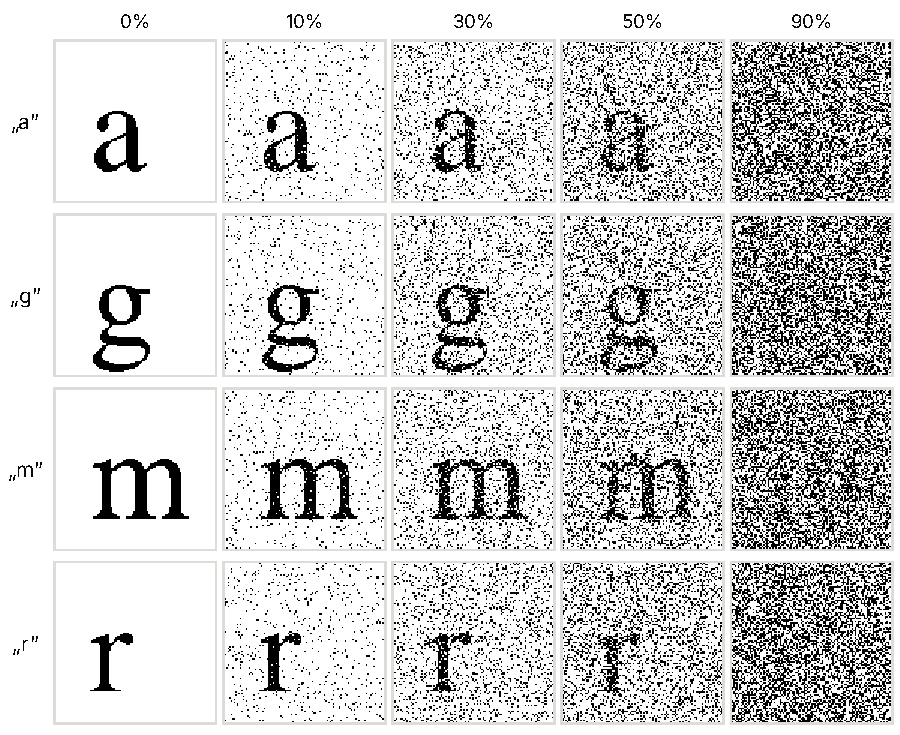
\includegraphics[width=0.85\linewidth]{fig_probki.pdf}
 \vspace{-0.2cm}
 \caption{Przykładowe obrazy testowe dla poziomów zaszumienia 0--90\%}
 \label{fig_probki}
\end{figure}

\subsubsection{Rezultat}

Początek raportu dla zaszumienia 30\% (format zgodny ze specyfikacją):
\begin{lstlisting}
letter a, noise level 30% -> letter a, noise level 0%, confidence: 0.449
letter b, noise level 30% -> letter b, noise level 0%, confidence: 0.497
letter c, noise level 30% -> letter c, noise level 0%, confidence: 0.400
\end{lstlisting}

\begin{table}[h!]
 \caption{Współczynnik pewności dla każdej litery; przy błędzie podano literę rozpoznaną (pogrubioną)}
 \centering
 \small
 \vspace{0.2cm}
 \begin{tabular}{c c c c c c}
  \hline\hline\\[-0.4cm]
  \textbf{Litera} & \textbf{0\%} & \textbf{10\%} & \textbf{30\%} & \textbf{50\%} & \textbf{90\%}\\[0.1cm]
  \hline
  \textbf{a} & $1{,}000$ & $0{,}688$ & $0{,}449$ & $0{,}311$ & \textbf{m}\,($0{,}210$) \\
  \textbf{b} & $1{,}000$ & $0{,}743$ & $0{,}497$ & $0{,}365$ & \textbf{m}\,($0{,}226$) \\
  \textbf{c} & $1{,}000$ & $0{,}666$ & $0{,}400$ & $0{,}292$ & \textbf{m}\,($0{,}214$) \\
  \textbf{d} & $1{,}000$ & $0{,}755$ & $0{,}497$ & $0{,}373$ & $0{,}231$ \\
  \textbf{e} & $1{,}000$ & $0{,}674$ & $0{,}428$ & $0{,}323$ & \textbf{m}\,($0{,}214$) \\
  \textbf{f} & $1{,}000$ & $0{,}662$ & $0{,}427$ & $0{,}300$ & \textbf{m}\,($0{,}209$) \\
  \textbf{g} & $1{,}000$ & $0{,}759$ & $0{,}505$ & $0{,}378$ & $0{,}223$ \\
  \textbf{h} & $1{,}000$ & $0{,}750$ & $0{,}503$ & $0{,}386$ & $0{,}227$ \\
  \textbf{i} & $1{,}000$ & $0{,}631$ & $0{,}373$ & $0{,}259$ & \textbf{m}\,($0{,}204$) \\
  \textbf{j} & $1{,}000$ & $0{,}692$ & $0{,}423$ & $0{,}319$ & \textbf{m}\,($0{,}204$) \\
  \textbf{k} & $1{,}000$ & $0{,}738$ & $0{,}486$ & $0{,}364$ & \textbf{m}\,($0{,}215$) \\
  \textbf{l} & $1{,}000$ & $0{,}637$ & $0{,}394$ & $0{,}280$ & \textbf{m}\,($0{,}216$) \\
  \textbf{m} & $1{,}000$ & $0{,}781$ & $0{,}545$ & $0{,}415$ & $0{,}242$ \\
  \textbf{n} & $1{,}000$ & $0{,}714$ & $0{,}480$ & $0{,}339$ & \textbf{m}\,($0{,}227$) \\
  \textbf{o} & $1{,}000$ & $0{,}687$ & $0{,}438$ & $0{,}307$ & \textbf{m}\,($0{,}213$) \\
  \textbf{p} & $1{,}000$ & $0{,}737$ & $0{,}506$ & $0{,}366$ & \textbf{m}\,($0{,}223$) \\
  \textbf{q} & $1{,}000$ & $0{,}743$ & $0{,}495$ & $0{,}372$ & \textbf{m}\,($0{,}215$) \\
  \textbf{r} & $1{,}000$ & $0{,}613$ & $0{,}370$ & $0{,}272$ & \textbf{m}\,($0{,}216$) \\
  \textbf{s} & $1{,}000$ & $0{,}642$ & $0{,}393$ & $0{,}272$ & \textbf{m}\,($0{,}207$) \\
  \textbf{t} & $1{,}000$ & $0{,}635$ & $0{,}393$ & $0{,}266$ & \textbf{m}\,($0{,}191$) \\
  \textbf{u} & $1{,}000$ & $0{,}709$ & $0{,}461$ & $0{,}344$ & \textbf{m}\,($0{,}226$) \\
  \textbf{v} & $1{,}000$ & $0{,}628$ & $0{,}380$ & $0{,}284$ & \textbf{m}\,($0{,}202$) \\
  \textbf{w} & $1{,}000$ & $0{,}736$ & $0{,}486$ & $0{,}364$ & \textbf{m}\,($0{,}217$) \\
  \textbf{x} & $1{,}000$ & $0{,}681$ & $0{,}425$ & $0{,}300$ & \textbf{m}\,($0{,}206$) \\
  \textbf{y} & $1{,}000$ & $0{,}687$ & $0{,}427$ & $0{,}314$ & \textbf{m}\,($0{,}204$) \\
  \textbf{z} & $1{,}000$ & $0{,}671$ & $0{,}405$ & $0{,}290$ & \textbf{m}\,($0{,}206$) \\
  \hline
  \textbf{popr.} & 26/26 & 26/26 & 26/26 & 26/26 & 4/26 \\
  \textbf{śr.} & $1{,}000$ & $0{,}695$ & $0{,}446$ & $0{,}325$ & $0{,}215$ \\[0.1cm]
  \hline
 \end{tabular}
 \label{tab_req}
\end{table}

\noindent Dla znaków niezaszumionych wszystkie 26 liter rozpoznano poprawnie
ze współczynnikiem pewności dokładnie $1{,}000$ (Tab.~\ref{tab_req}). Ten sam wynik daje
uruchomienie \texttt{madaline\_ocr.py training\_patterns training\_patterns}.
Potwierdza to poprawność implementacji: obraz identyczny ze wzorcem daje kąt zerowy.

Przy zaszumieniu 10\%, 30\% i~50\% również wszystkie litery rozpoznano poprawnie,
choć średnia pewność spadła z~$0{,}695$ do $0{,}325$. Litery z~liniami bardziej
cienkimi (np.~\texttt{i}, \texttt{r}, \texttt{t}) mają niższą pewność niż litery
,,ciężkie'' (np.~\texttt{m}, \texttt{g}), co zgadza się ze wzorem~(\ref{eq_theory}):
im mniejsze $n$, tym większy udział szumu w~wektorze wejściowym. Przy 90\% poprawnie
rozpoznano tylko 4 litery (\texttt{d}, \texttt{g}, \texttt{h}, \texttt{m}), a~aż 22
z~pozostałych rozpoznano jako \texttt{m}. Na obrazie widać już praktycznie sam szum
(Rys.~\ref{fig_probki}).

%%%%%%%%%%%%%%%%%%%%%%%%%%%%%%%%%%%%%%%%%%%%%%%%%%%%%%%%%%%%%%%%%%%%%%%%%%%%%%%%%%%%%%%%%%%%%%%%%%%%%%%%%%%%%%%%%
% PODROZDZIAŁ PT. EKSPERYMENT NR 2
%%%%%%%%%%%%%%%%%%%%%%%%%%%%%%%%%%%%%%%%%%%%%%%%%%%%%%%%%%%%%%%%%%%%%%%%%%%%%%%%%%%%%%%%%%%%%%%%%%%%%%%%%%%%%%%%%

\newpage
\subsection{Eksperyment nr 2 -- skuteczność w~funkcji poziomu szumu}

\subsubsection{Założenia}

Pojedyncze losowanie szumu w~eksperymencie nr~1 nie wystarcza, żeby oszacować
skuteczność przy wysokich poziomach. Dlatego dla poziomów 0--100\% (krok 10\%) wykonano
po 50 niezależnych losowań szumu dla każdej z~26 liter, czyli 1300 rozpoznań na poziom.
Te same funkcje co w~programach (\texttt{render\_letter}, \texttt{add\_noise},
\texttt{Madaline}) wywoływano bezpośrednio w~skrypcie \texttt{eksperymenty.py}.

\subsubsection{Przebieg}

Dla każdego rozpoznania zapisano: czy rozpoznanie jest poprawne, wyjście neuronu właściwej
litery oraz największe wyjście spośród pozostałych 25 neuronów. Wyniki porównano z~wartością
teoretyczną~(\ref{eq_theory}), uśrednioną po literach. Obliczono też macierz podobieństwa
wzorców $W W^{T}$ (Rys.~\ref{fig_podob}).

\subsubsection{Rezultat}

\begin{table}[h!]
 \caption{Wyniki 50 powtórzeń dla każdego poziomu szumu (26 liter)}
 \centering
 \setlength{\tabcolsep}{4pt}
 \small
 \vspace{0.2cm}
 \begin{tabular}{c c c c c l}
  \hline\hline\\[-0.4cm]
  \textbf{Szum} & \textbf{Skut. [\%]} & $\bar{y}_{\textrm{właściwy}}$ & \textbf{Wzór (\ref{eq_theory})} & $\bar{y}_{\textrm{max inny}}$ & \textbf{Najczęstsze błędy}\\[0.1cm]
  \hline
  0\% & $100{,}0$ & $1{,}000\pm0{,}000$ & $1{,}000$ & $0{,}729$ & -- \\
  10\% & $100{,}0$ & $0{,}692\pm0{,}050$ & $0{,}691$ & $0{,}513$ & -- \\
  20\% & $100{,}0$ & $0{,}542\pm0{,}053$ & $0{,}542$ & $0{,}411$ & -- \\
  30\% & $100{,}0$ & $0{,}447\pm0{,}050$ & $0{,}447$ & $0{,}348$ & -- \\
  40\% & $100{,}0$ & $0{,}378\pm0{,}046$ & $0{,}378$ & $0{,}302$ & -- \\
  50\% & $100{,}0$ & $0{,}325\pm0{,}042$ & $0{,}325$ & $0{,}269$ & -- \\
  60\% & $97{,}2$ & $0{,}281\pm0{,}037$ & $0{,}281$ & $0{,}244$ & r$\rightarrow$m, i$\rightarrow$m, r$\rightarrow$h \\
  70\% & $75{,}8$ & $0{,}245\pm0{,}033$ & $0{,}245$ & $0{,}228$ & i$\rightarrow$m, r$\rightarrow$m, c$\rightarrow$d \\
  80\% & $40{,}6$ & $0{,}214\pm0{,}030$ & $0{,}214$ & $0{,}218$ & i$\rightarrow$m, n$\rightarrow$m, z$\rightarrow$m \\
  90\% & $10{,}8$ & $0{,}186\pm0{,}026$ & $0{,}186$ & $0{,}213$ & a$\rightarrow$m, f$\rightarrow$m, i$\rightarrow$m \\
  100\% & $3{,}8$ & $0{,}161\pm0{,}023$ & $0{,}161$ & $0{,}211$ & a$\rightarrow$m, b$\rightarrow$m, c$\rightarrow$m \\
  \hline
 \end{tabular}
 \label{tab_sweep}
\end{table}

\begin{figure}[h!]
 \centering
 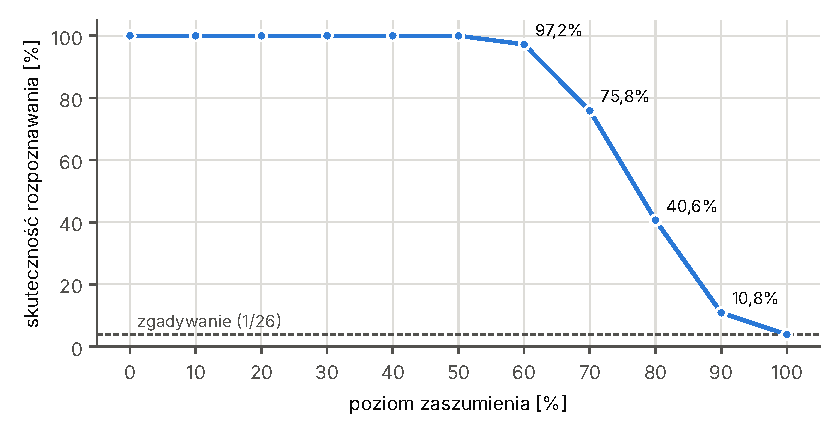
\includegraphics[width=11.5cm]{fig_skutecznosc.pdf}
 \vspace{-0.3cm}
 \caption{Skuteczność rozpoznawania w~funkcji poziomu zaszumienia}
 \label{fig_skut}
\end{figure}

\begin{figure}[h!]
 \centering
 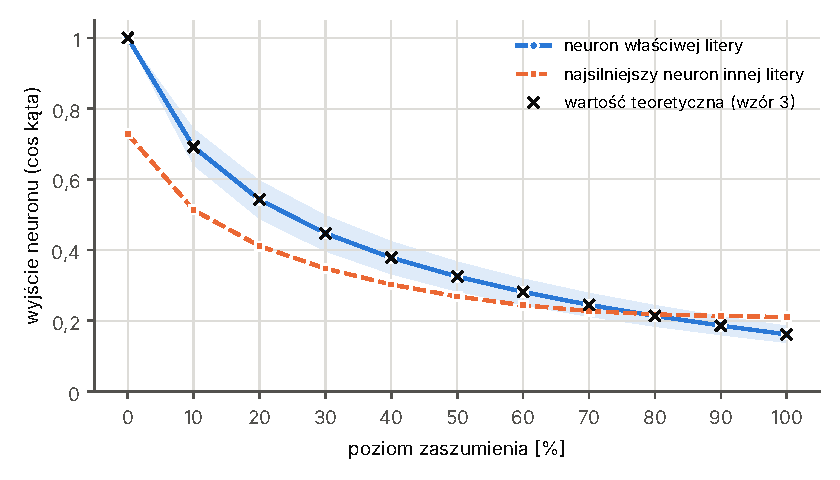
\includegraphics[width=11.5cm]{fig_wyjscia.pdf}
 \vspace{-0.3cm}
 \caption{Średnie wyjście neuronu właściwej litery ($\pm$ odchylenie standardowe),
 najsilniejszego neuronu innej litery oraz wartość ze wzoru~(\ref{eq_theory})}
 \label{fig_wyj}
\end{figure}

\noindent Sieć rozpoznaje bezbłędnie wszystkie litery aż do 50\% szumu (Tab.~\ref{tab_sweep},
Rys.~\ref{fig_skut}). Pierwsze błędy pojawiają się przy 60\% (skuteczność 97,2\%), a~potem
skuteczność szybko spada: 75,8\% przy 70\%, 40,6\% przy 80\% i~10,8\% przy 90\%. Przy 100\%
wynosi 3,8\%, czyli tyle, ile daje zgadywanie (1/26).

Wyjście neuronu właściwej litery jest zgodne ze wzorem~(\ref{eq_theory}) do trzeciego
miejsca po przecinku (Rys.~\ref{fig_wyj}). Współczynnik pewności nie jest więc
,,pewnością'' w~sensie probabilistycznym, tylko przewidywalną funkcją poziomu szumu
i~liczby pikseli litery. Już przy 10\% szumu spada do ok.~0,69, choć rozpoznanie jest
wciąż w~100\% poprawne. O~poprawności decyduje \textbf{różnica} między wyjściem właściwego
neuronu a~najsilniejszego konkurenta. Bez szumu wynosi ona $1-0{,}729$, bo średnio najbardziej
podobna inna litera ma cosinus $0{,}729$. Wraz ze wzrostem szumu różnica maleje, a~przy
ok.~75--80\% krzywe się przecinają. Odchylenie standardowe wyjścia ($\approx0{,}03$--$0{,}05$)
sprawia, że błędy zaczynają się nieco wcześniej, od 60\%.

\begin{figure}[h!]
 \centering
 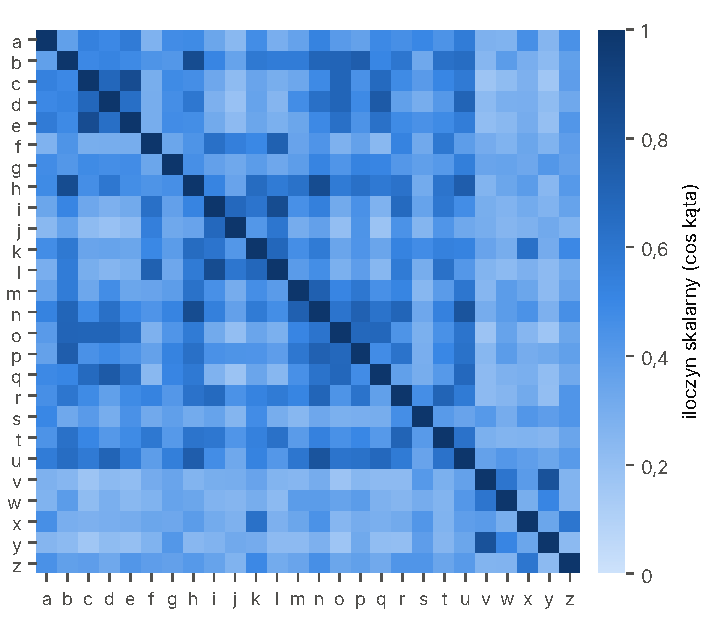
\includegraphics[width=10.5cm]{fig_podobienstwo.pdf}
 \vspace{-0.3cm}
 \caption{Podobieństwo (iloczyn skalarny) wzorców liter -- macierz $W W^{T}$}
 \label{fig_podob}
\end{figure}

Najbardziej podobne pary wzorców to \texttt{b}--\texttt{h} ($0{,}851$), \texttt{h}--\texttt{n}
($0{,}849$), \texttt{i}--\texttt{l} ($0{,}849$) i~\texttt{c}--\texttt{e} ($0{,}847$)
(Rys.~\ref{fig_podob}). Mimo to błędy przy dużym szumie nie dotyczą głównie tych par. Litery
przegrywają z~\texttt{m}, które ma najwięcej czarnych pikseli (1462, wobec 535 dla \texttt{i}).
Szum dodaje czarne piksele równomiernie na całym obrazie, a~wkład tych pikseli do wyjścia
neuronu $j$ rośnie jak $q\sqrt{n_j}$. Szum faworyzuje więc wzorce ,,ciężkie''. Pierwsze błędy
to cienkie litery: \texttt{r}$\rightarrow$\texttt{m}, \texttt{i}$\rightarrow$\texttt{m}, a~także
\texttt{c}$\rightarrow$\texttt{d}, bo \texttt{d} niemal zawiera kształt \texttt{c} i~ma więcej
pikseli. Przy 100\% szumu we wszystkich 2000 próbach wygrało \texttt{m}, zgodnie z~przewidywaniem
$\sqrt{n_j/2N}$ ze Wstępu teoretycznego.

%%%%%%%%%%%%%%%%%%%%%%%%%%%%%%%%%%%%%%%%%%%%%%%%%%%%%%%%%%%%%%%%%%%%%%%%%%%%%%%%%%%%%%%%%%%%%%%%%%%%%%%%%%%%%%%%%
% PODROZDZIAŁ PT. EKSPERYMENT NR 3
%%%%%%%%%%%%%%%%%%%%%%%%%%%%%%%%%%%%%%%%%%%%%%%%%%%%%%%%%%%%%%%%%%%%%%%%%%%%%%%%%%%%%%%%%%%%%%%%%%%%%%%%%%%%%%%%%

\newpage
\subsection{Eksperyment nr 3 -- przesunięcie litery i~zmiana kroju}

\subsubsection{Założenia}

Sieć porównuje obrazy piksel po pikselu, więc sprawdzono, jak reaguje na zmiany inne niż
szum. Znaki testowe były bez szumu, ale:
\begin{itemize}
 \item przesunięte w~poziomie o~1, 2, 4 lub 8 pikseli względem wzorca (parametr $x$),
 \item narysowane innym krojem o~tym samym rozmiarze: Liberation Serif (krój o~metryce
       zgodnej z~Times), DejaVu Serif (inny krój szeryfowy) i~Liberation Sans (bezszeryfowy).
\end{itemize}

\subsubsection{Przebieg}

Dla każdego wariantu rozpoznano 26 liter siecią zbudowaną z~wzorców Times bez przesunięcia.

\subsubsection{Rezultat}

\begin{table}[h!]
 \caption{Rozpoznawanie liter przesuniętych i~w~innym kroju (bez szumu)}
 \centering
 \setlength{\tabcolsep}{4pt}
 \small
 \vspace{0.2cm}
 \begin{tabular}{l c c c l}
  \hline\hline\\[-0.4cm]
  \textbf{Wariant} & \textbf{Skut. [\%]} & $\bar{y}_{\textrm{właściwy}}$ & $\bar{y}_{\textrm{zwycięzca}}$ & \textbf{Przykładowe błędy}\\[0.1cm]
  \hline
  przesunięcie o 1 px & $100{,}0$ & $0{,}891$ & $0{,}891$ & -- \\
  przesunięcie o 2 px & $96{,}2$ & $0{,}783$ & $0{,}784$ & r$\rightarrow$i \\
  przesunięcie o 4 px & $42{,}3$ & $0{,}577$ & $0{,}604$ & a$\rightarrow$u, b$\rightarrow$l, c$\rightarrow$u, \dots \\
  przesunięcie o 8 px & $3{,}8$ & $0{,}236$ & $0{,}414$ & a$\rightarrow$n, b$\rightarrow$f, c$\rightarrow$n, \dots \\
  Liberation Serif & $100{,}0$ & $0{,}763$ & $0{,}763$ & -- \\
  DejaVu Serif & $23{,}1$ & $0{,}433$ & $0{,}511$ & a$\rightarrow$o, b$\rightarrow$f, c$\rightarrow$t, \dots \\
  Liberation Sans & $38{,}5$ & $0{,}562$ & $0{,}624$ & a$\rightarrow$d, c$\rightarrow$u, d$\rightarrow$o, \dots \\
  \hline
 \end{tabular}
 \label{tab_rob}
\end{table}

\noindent Przesunięcie o~1~px nie powoduje błędów, ale obniża pewność do $0{,}891$
(Tab.~\ref{tab_rob}). Przy 4~px skuteczność spada do 42,3\%, a~przy 8~px do 3,8\%, czyli
poziomu zgadywania. Przesunięcie o~4~px bez żadnego szumu psuje więc rozpoznawanie bardziej
niż 70\% szumu losowego. Podobnie jest ze zmianą kroju. Liberation Serif, którego litery mają
prawie te same kształty i~szerokości co Times, rozpoznano w~100\% (pewność $0{,}763$).
Krój bezszeryfowy (38,5\%) i~DejaVu Serif o~innych proporcjach (23,1\%) rozpoznawane są już
słabo. Sieć MADALINE w~tej postaci jest dopasowaniem do szablonu: rozpoznaje dobrze tylko
znaki narysowane tym samym krojem i~w~tym samym miejscu co wzorce.

\section{Wnioski}

\begin{enumerate}
 \item Zaimplementowana sieć MADALINE działa poprawnie: znaki identyczne ze wzorcami
       rozpoznawane są zawsze ze współczynnikiem pewności dokładnie $1{,}000$.
 \item Sieć jest bardzo odporna na losowy szum pikseli. Przy 10\%, 30\% i~50\% szumu
       wszystkie 26 liter rozpoznano poprawnie (także w~50 powtórzeniach). Skuteczność spada
       dopiero powyżej 60\%, a~przy 90\% (10,8\%) zbliża się do poziomu zgadywania.
 \item Współczynnik pewności jest kosinusem kąta między wektorami i~maleje szybko nawet
       przy małym szumie (ok.~0,69 przy 10\%). Jego wartość dobrze przewiduje
       wzór~(\ref{eq_theory}). Niska pewność nie oznacza złego rozpoznania. O~wyniku decyduje
       przewaga właściwego neuronu nad najsilniejszym konkurentem.
 \item Przy dużym szumie sieć myli się w~sposób systematyczny: wybiera wzorce o~największej
       liczbie czarnych pikseli (tu \texttt{m}), bo losowe czarne piksele zwiększają
       podobieństwo do dużych wzorców. Przy obrazie całkowicie losowym wynik zależy już tylko
       od liczby pikseli wzorców.
 \item Słabością sieci jest brak odporności na przesunięcie i~zmianę kroju. Przesunięcie
       o~kilka pikseli albo inny krój czcionki szkodzą bardziej niż silny szum. W~praktyce
       przed rozpoznawaniem należałoby wyrównać położenie i~skalę znaku (np.~wyciąć
       i~przeskalować prostokąt otaczający literę) albo użyć wielu wzorców na jedną literę.
\end{enumerate}

%%%%%%%%%%%%%%%%%%%%%%%%%%%%%%%%%%%%%%%%%%%%%%%%%%%%%%%%%%%%%%%%%%%%%%%%%%%%%%%%%%%%%%%%%%%%%%%%%%%%%%%%%%%%%%%%%
% PODROZDZIAŁ PT. ZALACZNIKI
%%%%%%%%%%%%%%%%%%%%%%%%%%%%%%%%%%%%%%%%%%%%%%%%%%%%%%%%%%%%%%%%%%%%%%%%%%%%%%%%%%%%%%%%%%%%%%%%%%%%%%%%%%%%%%%%%

\section{Załączniki}

Pełny kod znajduje się w~plikach \texttt{font\_generator.py}, \texttt{madaline\_ocr.py},
\texttt{eksperymenty.py} i~\texttt{wykresy.py}. Poniżej podano najważniejsze fragmenty.

\noindent Szum (\texttt{font\_generator.py}):
\begin{lstlisting}[language=Python]
def add_noise(pixels, noise_level, rng):
    mask = rng.random(pixels.shape) < noise_level / 100
    noisy = pixels.copy()
    noisy[mask] = rng.integers(0, 2, size=int(mask.sum()))
    return noisy
\end{lstlisting}

\noindent Budowa sieci i~rozpoznawanie (\texttt{madaline\_ocr.py}):
\begin{lstlisting}[language=Python]
def image_to_vector(path):
    pixels = np.asarray(Image.open(path).convert("L")) < 128
    return pixels.astype(np.float64).ravel(), pixels.shape

def normalize(v):
    length = np.linalg.norm(v)
    return v / length if length > 0 else v

class Madaline:
    def __init__(self, weights, labels):
        self.W = weights            # wiersz l = znormalizowany wzorzec l
        self.labels = labels

    def outputs(self, x):
        return self.W @ x           # y_l = w(l) . x dla wszystkich neuronow

    def recognize(self, x):
        y = self.outputs(x)
        winner = int(np.argmax(y))
        return winner, float(y[winner])

# w main():
for x, test_label in zip(X, test_labels):
    winner, confidence = net.recognize(x)
    print(f"{test_label} -> {net.labels[winner]}, confidence: {confidence:.3f}")
\end{lstlisting}


%%%%%%%%%%%%%%%%%%%%%%%%%%%%%%%%%%%%%%%%%%%%%%%%%%%%%%%%%%%%%%%%%%%%%%%%%%%%%%%%%%%%%%%%%%%%%%%%%%%%%%%%%%%%%%%%%
% BIBLIOGRAFIA
%%%%%%%%%%%%%%%%%%%%%%%%%%%%%%%%%%%%%%%%%%%%%%%%%%%%%%%%%%%%%%%%%%%%%%%%%%%%%%%%%%%%%%%%%%%%%%%%%%%%%%%%%%%%%%%%%

\renewcommand\refname{Bibliografia}
\bibliographystyle{plain}
\bibliography{bibliografia}

\end{document}
